\documentclass{article}
\usepackage{tikz,amsmath,siunitx}
\usetikzlibrary{calc}
\usetikzlibrary{positioning}
\usetikzlibrary{arrows,snakes,backgrounds,patterns,matrix,shapes,fit,calc,shadows,plotmarks}
\usepackage[graphics,tightpage,active]{preview}
\PreviewEnvironment{tikzpicture}
\PreviewEnvironment{equation}
\PreviewEnvironment{equation*}
\newlength{\imagewidth}
\newlength{\imagescale}
\pagestyle{empty}
\thispagestyle{empty}
\begin{document}
\begin{tikzpicture} [auto, node distance=0cm]
\node at (0,0) (A){
    \begin{tikzpicture}
    \node[anchor=south west,inner sep=0] at (0,0) (foo) {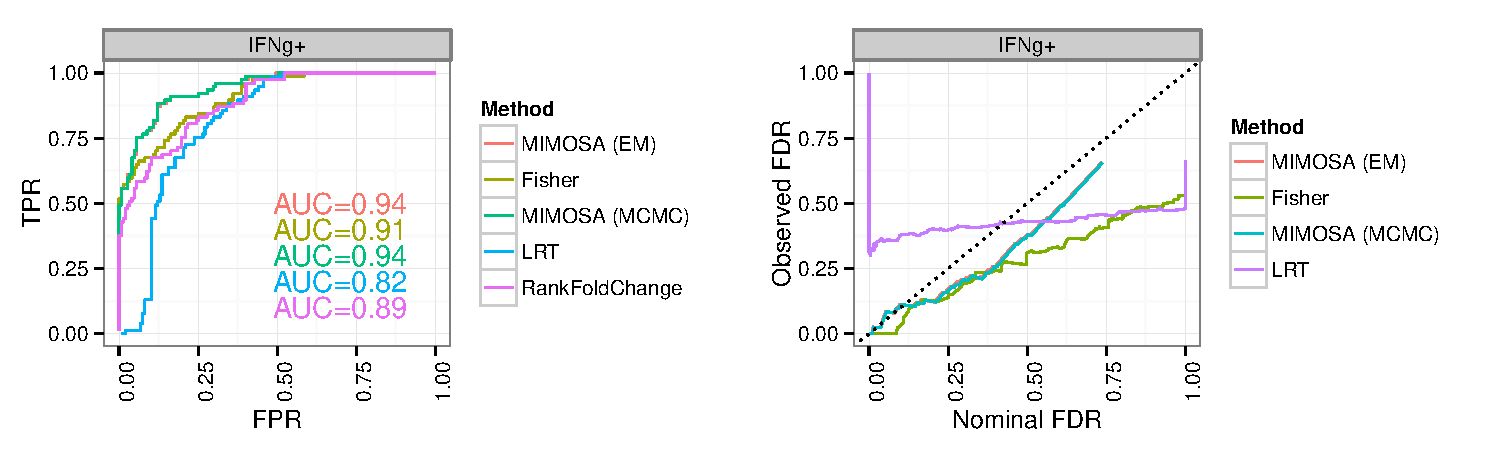
\includegraphics[width=\columnwidth]{Figures/revised_2.pdf}};
    \begin{scope}[x={(foo.south east)},y={(foo.north west)}]
    \node at (0,1) [font=\tiny\sffamily] {A} ;
    \node at (0.5,1) [font=\tiny\sffamily] {B} ;
    \end{scope}
\end{tikzpicture}
 };
 \node [below=of A] (B) {
 \begin{tikzpicture}
    \node[anchor=south west, inner sep=0] at (0,0) (bar){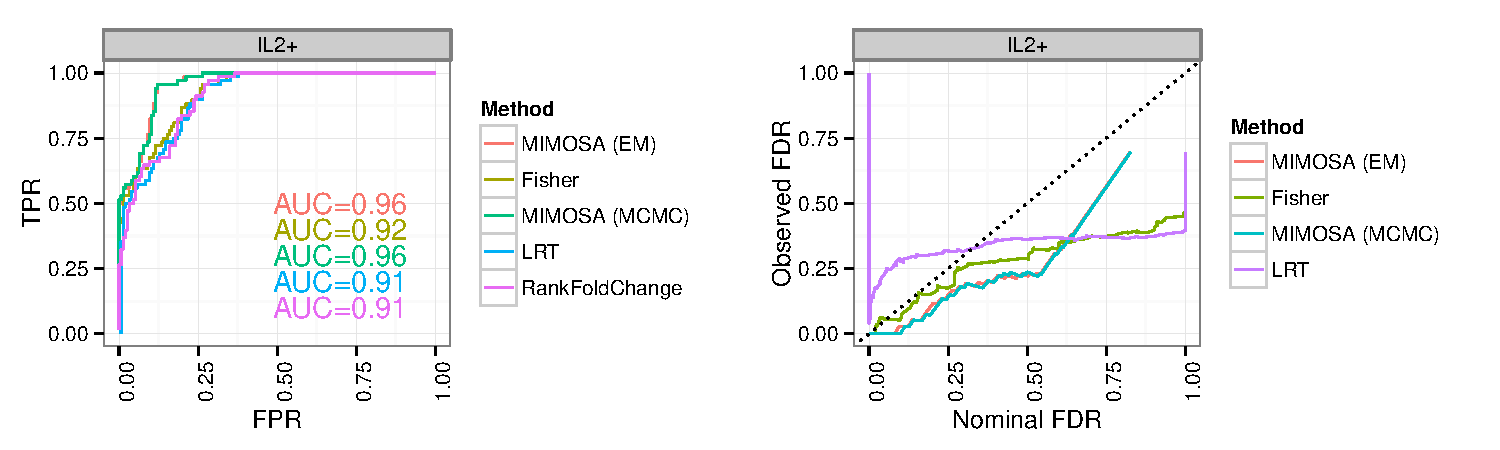
\includegraphics[width=\columnwidth]{Figures/revised_1.pdf}};
    \begin{scope} [x={(bar.south east)},y={(bar.north west)}]
    \node at (0,1) [font=\tiny\sffamily] {C} ;
    \node at (0.5,1) [font=\tiny\sffamily] {D} ;
    \end{scope}
    \end{tikzpicture}
 };
  \node [below=of B] (E) {
 \begin{tikzpicture}
    \node[anchor=south west, inner sep=0] at (0,0) (baz){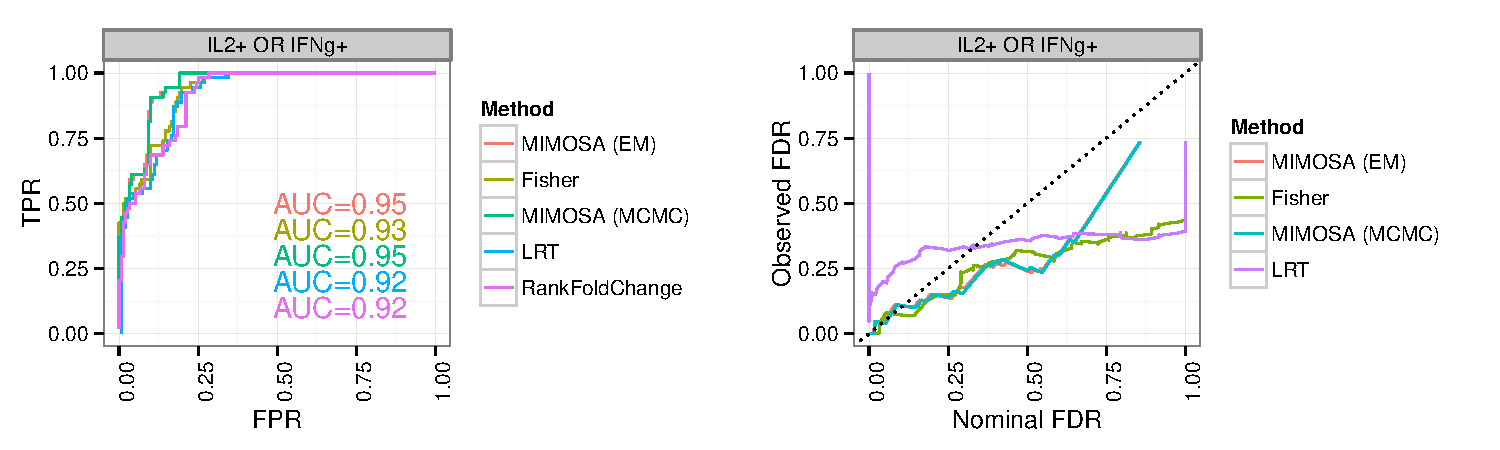
\includegraphics[width=\columnwidth]{Figures/revised_15.pdf}};
    \begin{scope} [x={(baz.south east)},y={(baz.north west)}]
    \node at (0,1) [font=\tiny\sffamily] {E} ;
    \node at (0.5,1) [font=\tiny\sffamily] {F} ;
    \end{scope}
    \end{tikzpicture}
 };
\end{tikzpicture}
\end{document}
